\chapter{Análisis}
\title{Análisis}
\label{cap:Analisis}

En este capitulo se realizará un análisis del proyecto para poder hacer así el futuro diseño del mismo.
Se describirán las diferentes partes que se han desarrollado.

\section{Análisis de Requisitos}
El análisis de los requisitos es el conjunto de todas las tareas que formarán las distintas necesidades de un software. Todos estos requisitos se tomarán por parte tanto del cliente como del desarrollador del proyecto ya que tiene que existir una viabilidad en el proyecto.

Se realiza un análisis de requisitos para que al llegar a la fase de diseño se tenga un software óptimo, sin contradicciones o sin ambigüedades, por ejemplo.

Los requisitos se van generando a partir de las diferentes entrevista que se tienen con el cliente.

\subsection{Requisitos Funcionales}
\begin{itemize}
  \item \textbf{RF-1:} Conectarse a un servidor INDI.
  \item \textbf{RF-2:} Mostrar todos los dispositivos conectados en el servidor INDI.
  \item \textbf{RF-3:} Obtener las propiedades de los dispositivos conectados.
  \item \textbf{RF-4:} Agrupar las propiedades de los dispositivos por diferentes grupos.
  \item \textbf{RF-5:} Editar las diferentes propiedades de INDI:
  \begin{itemize}
    \item \textbf{RF-5.1:} Propiedad Text.
    \item \textbf{RF-5.2:} Propiedad Number.
    \item \textbf{RF-5.3:} Propiedad Switch.
    \item \textbf{RF-5.4:} Propiedad Blob.
  \end{itemize}
  \item \textbf{RF-6:} Activar la recepción de Blob en cada dispositivo conectado.
  \item \textbf{RF-7:} Desactivar la recepción de Blob en cada dispositivo conectado.
\end{itemize}

\subsection{Requisitos No Funcionales}
\begin{itemize}
  \item \textbf{RNF-1:} Utilización de licencias libres y herramientas de desarrollo del proyecto de Software Libre para publicar el proyecto como tal.
  \item \textbf{RNF-2:} El sistema solamente podrá conectarse con dispositivos que se encuentren conectados físicamente con el servidor.
  \item \textbf{RNF-3:} Solamente se mostrarán las interfaces de los dispositivos de los cuales se hayan obtenido sus propiedades mediante el fichero XML.
  \item \textbf{RNF-4:} Se deben emplear los estándares de los diferentes lenguajes.
\end{itemize}

\section{Descripción de Actores}
Los actores son los personajes que participarán en el sistema. Tendrán a su disposición todas las funciones del sistema para poder interactuar con él.

A continuación se detalla el único usuario que tendrá el sistema:\\ \\
\textbf{AC-1: Usuario}
\begin{itemize}
  \item \textbf{Descripción:} Persona que utilizará el prototipo de cliente realizando con él las distintas funcionalidades que posee.
  \item \textbf{Características:} Es el único usuario del sistema y el que llevará a cabo todas las acciones.
  \item \textbf{Relaciones:} Ninguna.
  \item \textbf{Atributos:} Ninguno.
  \item \textbf{Comentarios:} El usuario tiene la responsabilidad de hacer una buena utilización del prototipo de cliente. Deberá tener, en mayor o menor medida, conocimientos sobre la Astronomía, pues el manejo del prototipo de cliente web se ha diseñado para trabajar con él, tanto a nivel profesional como a nivel \textit{amateur}.
\end{itemize}

\section{Descripción de Casos de Uso}
Los diferentes casos de uso nos permiten conocer como los actores se desenvuelven en el sistema, es decir, las diferentes funcionalidades que tienen disponibles en el sistema.\\


\subsection{\textbf{CU-1: Conectarse a un servidor y obtener los diferentes dispositivos}}
\begin{itemize}
  \item \textbf{Actores:} Usuario (I)
  \item \textbf{Tipo:} Primario, Esencial
  \item \textbf{Precondición:}
  \item \textbf{Postcondición:} Se realiza la conexión con el servidor.
  \item \textbf{Propósito:} Conectarse a un servidor.
  \item \textbf{Resumen:} El usuario se conectará a un servidor mediante su IP y puerto correspondiente.
  \item \textbf{Autor:} Pablo Torrecillas Ortega
  \item \textbf{Versión:} 1.0
  \begin{table}[!ht]
      \begin{center}
	\begin{tabular}{|l|l|l|l|}
	  \hline
	  \multicolumn{4}{|c|}{{\bf Curso normal}}
	  \\ \hline
	  \multicolumn{2}{|c|}{{\bf Actor}} & \multicolumn{2}{c|}{{\bf Sistema}}
	  \\ \hline
	  {\it 1} &
	  \begin{tabular}[c]{@{}l@{}}
	    Usuario: Introduce la IP \\
	    y el puerto y pulsa sobre\\
      el botón conectar.\\
	  \end{tabular} &
	  &
	  \\ \hline
	  &
	  &
	  {\it 2} &
	  \begin{tabular}[c]{@{}l@{}}
	    El sistema almacena la IP\\
	    y el puerto.\\
      Seguidamente, muestra los\\
      Dispositivos conectados.
	  \end{tabular}
	  \\ \hline
	\end{tabular}
	\caption{CU-1. Conectarse a un servidor y obtener los diferentes dispositivos}
	\label{table:CU_1}
      \end{center}
    \end{table}
\end{itemize}



\subsection{\textbf{CU-2: Finalizar la aplicación}}
\begin{itemize}
  \item \textbf{Actores:} Usuario (I)
  \item \textbf{Tipo:} Secundario, Esencial
  \item \textbf{Precondición:} Que esté abierta la ventana del prototipo de cliente.
  \item \textbf{Postcondición:} Finalizará la conexión con los dispositivos del servidor.
  \item \textbf{Propósito:} Finalizar la aplicación.
  \item \textbf{Resumen:} El usuario finaliza la aplicación cerrando la conexión con el servidor.
  \item \textbf{Autor:} Pablo Torrecillas Ortega
  \item \textbf{Versión:} 1.0
  \begin{table}[!ht]
      \begin{center}
  \begin{tabular}{|l|l|l|l|}
    \hline
    \multicolumn{4}{|c|}{{\bf Curso normal}}
    \\ \hline
    \multicolumn{2}{|c|}{{\bf Actor}} & \multicolumn{2}{c|}{{\bf Sistema}}
    \\ \hline
    {\it 1} &
    \begin{tabular}[c]{@{}l@{}}
      Usuario: Cierra la ventana \\
      del navegador.\\
    \end{tabular} &
    &
    \\ \hline
    &
    &
    {\it 2} &
    \begin{tabular}[c]{@{}l@{}}
      El sistema cierra el navegador\\
      de cliente y finaliza la\\
      aplicación.\\
    \end{tabular}
    \\ \hline
  \end{tabular}
  \caption{CU-2. Finalizar la aplicación}
  \label{table:CU_2}
      \end{center}
    \end{table}
\end{itemize}




\subsection{\textbf{CU-3: Mostrar un dispositivo}}
\begin{itemize}
  \item \textbf{Actores:} Usuario (I)
  \item \textbf{Tipo:} Primario, Esencial
  \item \textbf{Precondición:} Que exista una conexión previamente bien realizada.
  \item \textbf{Postcondición:} Se mostrará la ventana de un dispositivo concreto.
  \item \textbf{Propósito:} Mostrar un dispositivo en el navegador.
  \item \textbf{Resumen:} EL usuario seleccionará un dispositivo concreto del conjunto de ventanas de dispositivos.
  \item \textbf{Autor:} Pablo Torrecillas Ortega
  \item \textbf{Versión:} 1.0
  \begin{table}[!ht]
      \begin{center}
  \begin{tabular}{|l|l|l|l|}
    \hline
    \multicolumn{4}{|c|}{{\bf Curso normal}}
    \\ \hline
    \multicolumn{2}{|c|}{{\bf Actor}} & \multicolumn{2}{c|}{{\bf Sistema}}
    \\ \hline
    {\it 1} &
    \begin{tabular}[c]{@{}l@{}}
      Usuario: Selecciona una ventana \\
      del conjunto de ventanas de\\
      dispositivos para mostrar todas\\
      sus propiedades y trabajar\\
      con él.\\
    \end{tabular} &
    &
    \\ \hline
    &
    &
    {\it 2} &
    \begin{tabular}[c]{@{}l@{}}
      El sistema muestra la \\
      ventana seleccionada.\\
    \end{tabular}
    \\ \hline
  \end{tabular}
  \caption{CU-3. Mostrar un dispositivo}
  \label{table:CU_3}
      \end{center}
    \end{table}
\end{itemize}


\subsection{\textbf{CU-4: Editar la propiedad \textit{text}}}
\begin{itemize}
  \item \textbf{Actores:} Usuario (I)
  \item \textbf{Tipo:} Primario, Esencial
  \item \textbf{Precondición:} Que exista un dispositivo conectado con el servidor y con una propiedad \textit{text} que se pueda modificar.
  \item \textbf{Postcondición:} Se modificará la propiedad \textit{text} y se enviará el valor al servidor.
  \item \textbf{Propósito:} Editar la propiedad \textit{text}.
  \item \textbf{Resumen:} El usuario modificará una propiedad \textit{text} en su correspondiente cuadro de modificación.
  \item \textbf{Autor:} Pablo Torrecillas Ortega
  \item \textbf{Versión:} 1.0
  \begin{table}[!ht]
      \begin{center}
	\begin{tabular}{|l|l|l|l|}
	  \hline
	  \multicolumn{4}{|c|}{{\bf Curso normal}}
	  \\ \hline
	  \multicolumn{2}{|c|}{{\bf Actor}} & \multicolumn{2}{c|}{{\bf Sistema}}
	  \\ \hline
	  {\it 1} &
	  \begin{tabular}[c]{@{}l@{}}
	    Usuario: Pulsa el cuadro\\
	    de modificación del texto.\\
	  \end{tabular} &
	  &
	  \\ \hline
	  {\it 2} &
    \begin{tabular}[c]{@{}l@{}}
	    Usuario: Escribe el valor\\
	    de texto a modificar y \\
      pulsa el botón actualizar\\
	  \end{tabular}
	  &
	  &
	  \\ \hline
	  &
	  &
	  {\it 3}&
    \begin{tabular}[c]{@{}l@{}}
      El sistema cambia el \\
      valor del texto y lo\\
      envía al servidor.\\
	  \end{tabular}
	  \\ \hline
	\end{tabular}
	\caption{CU-4. Editar la propiedad \textit{text}}
	\label{table:CU_4}
      \end{center}
    \end{table}
\end{itemize}



\subsection{\textbf{CU-5: Editar la propiedad \textit{number}}}
\begin{itemize}
  \item \textbf{Actores:} Usuario (I)
  \item \textbf{Tipo:} Primario, Esencial
  \item \textbf{Precondición:} Que exista un dispositivo conectado con el servidor y con una propiedad \textit{number} que se pueda modificar.
  \item \textbf{Postcondición:} Se modificará la propiedad \textit{number} y se enviará el valor al servidor.
  \item \textbf{Propósito:} Editar la propiedad \textit{number}.
  \item \textbf{Resumen:} El usuario modificará una propiedad \textit{number} en su correspondiente cuadro de modificación.
  \item \textbf{Autor:} Pablo Torrecillas Ortega
  \item \textbf{Versión:} 1.0
  \begin{table}[!ht]
      \begin{center}
  \begin{tabular}{|l|l|l|l|}
    \hline
    \multicolumn{4}{|c|}{{\bf Curso normal}}
    \\ \hline
    \multicolumn{2}{|c|}{{\bf Actor}} & \multicolumn{2}{c|}{{\bf Sistema}}
    \\ \hline
    {\it 1} &
    \begin{tabular}[c]{@{}l@{}}
      Usuario: Pulsa el cuadro\\
      de modificación de la\\
      propiedad numérica\\
    \end{tabular} &
    &
    \\ \hline
    {\it 2} &
    \begin{tabular}[c]{@{}l@{}}
      Usuario: Escribe el valor\\
      del número a modificar y \\
      pulsa el botón actualizar\\
    \end{tabular}
    &
    &
    \\ \hline
    &
    &
    {\it 3}&
    \begin{tabular}[c]{@{}l@{}}
      El sistema cambia el \\
      valor del número y lo\\
      envía al servidor.\\
    \end{tabular}
    \\ \hline
  \end{tabular}
  \caption{CU-5. Editar la propiedad \textit{number}}
  \label{table:CU_5}
      \end{center}
    \end{table}
\end{itemize}



\subsection{\textbf{CU-6: Editar la propiedad \textit{switch}}}
\begin{itemize}
  \item \textbf{Actores:} Usuario (I)
  \item \textbf{Tipo:} Primario, Esencial
  \item \textbf{Precondición:} Que exista un dispositivo conectado con el servidor y con una propiedad \textit{switch} que se pueda modificar.
  \item \textbf{Postcondición:} Se modificará la propiedad \textit{switch} y se enviará el valor al servidor.
  \item \textbf{Propósito:} Editar la propiedad \textit{switch}.
  \item \textbf{Resumen:} El usuario modificará una propiedad \textit{switch} en su correspondiente cuadro de modificación.
  \item \textbf{Autor:} Pablo Torrecillas Ortega
  \item \textbf{Versión:} 1.0
  \begin{table}[!ht]
      \begin{center}
  \begin{tabular}{|l|l|l|l|}
    \hline
    \multicolumn{4}{|c|}{{\bf Curso normal}}
    \\ \hline
    \multicolumn{2}{|c|}{{\bf Actor}} & \multicolumn{2}{c|}{{\bf Sistema}}
    \\ \hline
    {\it 1} &
    \begin{tabular}[c]{@{}l@{}}
      Usuario: Selecciona una o \\
      muchas de las opciones\\
      dependiendo del tipo de switch\\
      que sea.\\
    \end{tabular} &
    &
    \\ \hline
    &
    &
    {\it 2} &
    \begin{tabular}[c]{@{}l@{}}
      El sistema muestra la o las\\
      opciones seleccionadas y envía\\
      los valores al servidor.\\
    \end{tabular}
    \\ \hline
  \end{tabular}
  \caption{CU-6. Editar la propiedad \textit{switch}}
  \label{table:CU_6}
      \end{center}
    \end{table}
\end{itemize}



\subsection{\textbf{CU-7: Editar la propiedad \textit{blob}}}
\begin{itemize}
  \item \textbf{Actores:} Usuario (I)
  \item \textbf{Tipo:} Primario, Esencial
  \item \textbf{Precondición:} Que exista un dispositivo conectado con el servidor y con una propiedad \textit{blob} que se pueda modificar.
  \item \textbf{Postcondición:} Se modificará la propiedad \textit{blob} y se enviará el valor al servidor.
  \item \textbf{Propósito:} Editar la propiedad \textit{blob}.
  \item \textbf{Resumen:} El usuario modificará una propiedad \textit{blob} en su correspondiente cuadro de modificación.
  \item \textbf{Autor:} Pablo Torrecillas Ortega
  \item \textbf{Versión:} 1.0
  \begin{table}[!ht]
      \begin{center}
  \begin{tabular}{|l|l|l|l|}
    \hline
    \multicolumn{4}{|c|}{{\bf Curso normal}}
    \\ \hline
    \multicolumn{2}{|c|}{{\bf Actor}} & \multicolumn{2}{c|}{{\bf Sistema}}
    \\ \hline
    {\it 1} &
    \begin{tabular}[c]{@{}l@{}}
      Usuario: Selecciona la  \\
      propiedad que desea desactivar.\\
    \end{tabular} &
    &
    \\ \hline
    &
    &
    {\it 2} &
    \begin{tabular}[c]{@{}l@{}}
      El sistema muestra la\\
      propiedad modificada y \\
      enviar los valores al\\
      servidor.\\
    \end{tabular}
    \\ \hline
  \end{tabular}
  \caption{CU-7. Editar la propiedad \textit{blob}}
  \label{table:CU_7}
      \end{center}
    \end{table}
\end{itemize}



\subsection{\textbf{CU-8: Activar la recepción de \textit{blob}}}
\begin{itemize}
  \item \textbf{Actores:} Usuario (I)
  \item \textbf{Tipo:} Secundario, Esencial
  \item \textbf{Precondición:} Que exista un dispositivo conectado con el servidor.
  \item \textbf{Postcondición:} Se activará la recepción de \textit{blob}
  \item \textbf{Propósito:} Activar blob
  \item \textbf{Resumen:} El usuario activará la recepción de \textit{blob} de un dispositivo concreto que por defecto viene desactivada
  \item \textbf{Autor:} Pablo Torrecillas Ortega
  \item \textbf{Versión:} 1.0
  \begin{table}[!ht]
      \begin{center}
  \begin{tabular}{|l|l|l|l|}
    \hline
    \multicolumn{4}{|c|}{{\bf Curso normal}}
    \\ \hline
    \multicolumn{2}{|c|}{{\bf Actor}} & \multicolumn{2}{c|}{{\bf Sistema}}
    \\ \hline
    {\it 1} &
    \begin{tabular}[c]{@{}l@{}}
      Usuario: Pulsa el botón  \\
      de recepción de \textit{blob}\\
      de un dispositivo concreto.\\
    \end{tabular} &
    &
    \\ \hline
    &
    &
    {\it 2} &
    \begin{tabular}[c]{@{}l@{}}
      El sistema deja seleccionado\\
      el botón y envia al servidor \\
      el mensaje oportuno para activar \\
      la recepción de BLOB.\\
    \end{tabular}
    \\ \hline
  \end{tabular}
  \caption{CU-8. Activar la recepción de \textit{blob}}
  \label{table:CU_8}
      \end{center}
    \end{table}
\end{itemize}



\subsection{\textbf{CU-9: Desactivar la recepción de \textit{blob}}}
\begin{itemize}
  \item \textbf{Actores:} Usuario (I)
  \item \textbf{Tipo:} Secundario, Esencial
  \item \textbf{Precondición:} Que exista un dispositivo conectado al servidor y tenga activada la recepción de \textit{blob}.
  \item \textbf{Postcondición:} Se desactivará la recepción de \textit{blob} para ese dispositivo.
  \item \textbf{Propósito:} Desactivar la recepción de \textit{blob}.
  \item \textbf{Resumen:} El usuario desactivará la recepción de \textit{blob} de un dispositivo concreto que tenía activada la recepción.
  \item \textbf{Autor:} Pablo Torrecillas Ortega
  \item \textbf{Versión:} 1.0
  \begin{table}[!ht]
      \begin{center}
  \begin{tabular}{|l|l|l|l|}
    \hline
    \multicolumn{4}{|c|}{{\bf Curso normal}}
    \\ \hline
    \multicolumn{2}{|c|}{{\bf Actor}} & \multicolumn{2}{c|}{{\bf Sistema}}
    \\ \hline
    {\it 1} &
    \begin{tabular}[c]{@{}l@{}}
      Usuario: Pulsa el botón para  \\
      desactivar la recepción.\\
    \end{tabular} &
    &
    \\ \hline
    &
    &
    {\it 2} &
    \begin{tabular}[c]{@{}l@{}}
      El sistema desmarca\\
      el botón y envia al servidor \\
      el mensaje oportuno para\\
      desactivar la recepción de BLOB.\\
    \end{tabular}
    \\ \hline
  \end{tabular}
  \caption{CU-9. Desactivar la recepción de \textit{blob}}
  \label{table:CU_9}
      \end{center}
    \end{table}
\end{itemize}



\subsection{\textbf{CU-10: Guardar un \textit{blob}}}
\begin{itemize}
  \item \textbf{Actores:} Usuario (I)
  \item \textbf{Tipo:} Secundario, Esencial
  \item \textbf{Precondición:} Que exista al menos un dispositivo conectado en el servidor y tenga activada la recepción de \textit{blob}.
  \item \textbf{Postcondición:} Se almacenará un \textit{blob} en la memoria de la máquina.
  \item \textbf{Propósito:} Guardar un \textit{blob}
  \item \textbf{Resumen:} El usuario guardará un \textit{blob} en la memoria para poder hacer uso de él.
  \item \textbf{Autor:} Pablo Torrecillas Ortega
  \item \textbf{Versión:} 1.0
  \begin{table}[!ht]
      \begin{center}
  \begin{tabular}{|l|l|l|l|}
    \hline
    \multicolumn{4}{|c|}{{\bf Curso normal}}
    \\ \hline
    \multicolumn{2}{|c|}{{\bf Actor}} & \multicolumn{2}{c|}{{\bf Sistema}}
    \\ \hline
    {\it 1} &
    \begin{tabular}[c]{@{}l@{}}
      Usuario: Pulsa el botón para  \\
      guardar un \textit{blob}.\\
    \end{tabular} &
    &
    \\ \hline
    &
    &
    {\it 2} &
    \begin{tabular}[c]{@{}l@{}}
      El sistema almacena\\
      la información proporcionada\\
      por el \textit{blob}. \\
    \end{tabular}
    \\ \hline
  \end{tabular}
  \caption{CU-10. Guardar un \textit{blob}}
  \label{table:CU_10}
      \end{center}
    \end{table}
\end{itemize}



\subsection{\textbf{CU-11: Cambiar de grupo de propiedades}}
\begin{itemize}
  \item \textbf{Actores:} Usuario (I)
  \item \textbf{Tipo:} Primario, Esencial
  \item \textbf{Precondición:} Que exista un dispositivo conectado al servidor y que tenga al menos dos grupos de propiedades.
  \item \textbf{Postcondición:} Se cambiará la vista de la pestaña según los elementos que tenga.
  \item \textbf{Propósito:} Cambiar de grupo de propiedades.
  \item \textbf{Resumen:} El usuario cambiará de pestaña en la ventana de un dispositivo.
  \item \textbf{Autor:} Pablo Torrecillas Ortega
  \item \textbf{Versión:} 1.0
  \begin{table}[!ht]
      \begin{center}
  \begin{tabular}{|l|l|l|l|}
    \hline
    \multicolumn{4}{|c|}{{\bf Curso normal}}
    \\ \hline
    \multicolumn{2}{|c|}{{\bf Actor}} & \multicolumn{2}{c|}{{\bf Sistema}}
    \\ \hline
    {\it 1} &
    \begin{tabular}[c]{@{}l@{}}
      Usuario: Pulsa el nombre de\\
      la pestaña para cambiar de\\
      grupo de propiedades.\\
    \end{tabular} &
    &
    \\ \hline
    &
    &
    {\it 2} &
    \begin{tabular}[c]{@{}l@{}}
      El sistema muestra la \\
      pestaña seleccionada con\\
      el conjunto de propiedades\\
      que ésta posee.\\
    \end{tabular}
    \\ \hline
  \end{tabular}
  \caption{CU-11. Cambiar de grupo de propiedades}
  \label{table:CU_11}
      \end{center}
    \end{table}
\end{itemize}



\subsection{\textbf{CU-12: Cerrar un dispositivo}}
\begin{itemize}
  \item \textbf{Actores:} Usuario (I)
  \item \textbf{Tipo:} Secundario, Esencial
  \item \textbf{Precondición:} Que exista al menos un dispositivo conectado en el servidor.
  \item \textbf{Postcondición:} Se cerrará el dispositio y no se podrá trabajar con él a menos que se vuelva a realizar la conexión.
  \item \textbf{Propósito:} Cerrar un dispositivo.
  \item \textbf{Resumen:} El usuario cerrará un dispositivo que está conectado con el servidor eliminando la posibilidad de realizar más acciones con él.
  \item \textbf{Autor:} Pablo Torrecillas Ortega
  \item \textbf{Versión:} 1.0
  \begin{table}[!ht]
      \begin{center}
  \begin{tabular}{|l|l|l|l|}
    \hline
    \multicolumn{4}{|c|}{{\bf Curso normal}}
    \\ \hline
    \multicolumn{2}{|c|}{{\bf Actor}} & \multicolumn{2}{c|}{{\bf Sistema}}
    \\ \hline
    {\it 1} &
    \begin{tabular}[c]{@{}l@{}}
      Usuario: Pulsa sobre el botón\\
      X de la ventana del dispositivo\\
      para cerrarlo\\
    \end{tabular} &
    &
    \\ \hline
    &
    &
    {\it 2} &
    \begin{tabular}[c]{@{}l@{}}
      El sistema cierra le ventana\\
      del dispositivo que se ha \\
      seleccionado.\\
    \end{tabular}
    \\ \hline
  \end{tabular}
  \caption{CU-12. Cerrar un dispositivo}
  \label{table:CU_12}
      \end{center}
    \end{table}
\end{itemize}


\section{Diagrama de Casos de Uso}
Los diagramas de casos de uso sirven para especificar la comunicación y comportamiento de un sistema mediante su interacción con los usuarios y/u otros sistemas.\\
Los diagramas de casos de uso, se utilizan también para ilustrar los requerimientos del sistema al mostrar cómo reacciona a eventos que se producen en su ámbito o en él mismo \cite{CasosUso}.

\begin{figure}[htb]
\centering
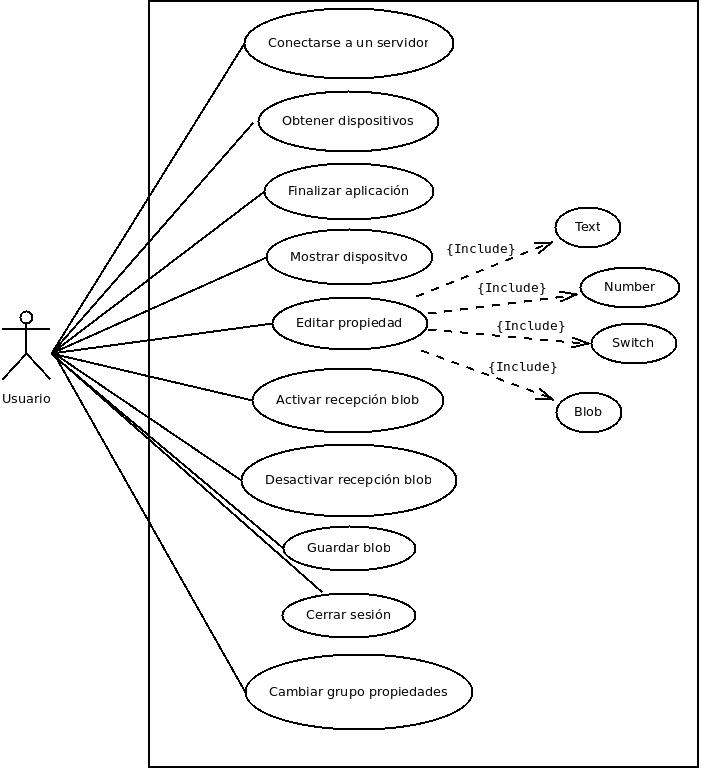
\includegraphics[width=0.9\textwidth]{./imagenes/DiagramaCasosUsoFinal}
\caption{Diagrama de Casos de Uso} \label{fig:DiagramaCasosUsoFinal}
\end{figure}
